\documentclass[12pt,a4paper]{article}

% ---------------------------------------------------------------
%  Course End Project Report - Airline Reservation System
%  Compile with:  pdflatex main.tex  (run twice for the contents)
% ---------------------------------------------------------------
\usepackage[T1]{fontenc}
\usepackage[a4paper,margin=1in]{geometry}
\usepackage[strings]{underscore}
\usepackage{graphicx,xcolor,float,booktabs,longtable,array,tabularx}
\usepackage{amsmath,enumitem,adjustbox,pdflscape,caption,tocloft}
\usepackage{listings}
\usepackage{tikz}
\usetikzlibrary{shapes.geometric,shapes.multipart,arrows.meta,calc,positioning}
\usepackage[hidelinks]{hyperref}

\captionsetup{font=small}
\setlength{\parindent}{1.2em}
\setlength{\parskip}{0.3em}
\renewcommand{\arraystretch}{1.15}
\renewcommand{\cftsecleader}{\cftdotfill{\cftdotsep}}
\renewcommand{\cftsecfont}{\normalfont}
\renewcommand{\cftsecpagefont}{\normalfont}

% ---------- listing styles ----------
\lstdefinestyle{code}{
  language=SQL, sensitive=false,
  morekeywords={FUNCTION,PROCEDURE,TRIGGER,BEGIN,END,DECLARE,CURSOR,IF,THEN,
    ELSE,ELSIF,LOOP,RETURN,EXCEPTION,WHEN,REPLACE,FOR,EACH,ROW,NUMBER,
    VARCHAR2,INSERTING,UPDATING,DELETING,SAVEPOINT,COMMIT,ROLLBACK,
    RAISE_APPLICATION_ERROR,RAISE,OTHERS,NO_DATA_FOUND,IDENTITY,GENERATED,
    ALWAYS,ORGANIZATION,EXPLAIN,PLAN,TRUNC,SYSDATE,USER,LEFT,JOIN,ON,
    CASE,SERVEROUTPUT},
  basicstyle=\ttfamily\footnotesize, keywordstyle=\color{blue!60!black}\bfseries,
  commentstyle=\color{green!40!black}\itshape, stringstyle=\color{red!50!black},
  morecomment=[l]{--}, breaklines=true, columns=fullflexible, keepspaces=true,
  frame=single, rulecolor=\color{black!30}, backgroundcolor=\color{black!3},
  showstringspaces=false, upquote=true, aboveskip=6pt, belowskip=4pt
}
\lstdefinestyle{term}{
  language={}, basicstyle=\ttfamily\scriptsize\color{white},
  backgroundcolor=\color{black!90}, columns=fixed, keepspaces=true,
  breaklines=true, frame=none, xleftmargin=6pt, framexleftmargin=6pt,
  framextopmargin=5pt, framexbottommargin=5pt, upquote=true,
  aboveskip=4pt, belowskip=2pt
}
\lstnewenvironment{terminal}{\lstset{style=term}}{}
\lstnewenvironment{code}{\lstset{style=code}}{}
\newcommand{\sqlfile}{\begingroup\catcode`\_=12 \sqlfileA}
\newcommand{\sqlfileA}[1]{\lstinputlisting[style=code]{sql/#1}\endgroup}

\newcommand{\pk}[1]{\textit{\underline{#1}}}
\newcommand{\fk}[1]{#1\textsuperscript{FK}}

\begin{document}

% ================================================================
%                           COVER PAGE
% ================================================================
\begin{titlepage}
\thispagestyle{empty}
\centering
\vspace*{0.5cm}


\begin{center}

\includegraphics[width=5.00cm]{VMEG_LOGO.png}
\end{center}

\vspace{0.8cm}

{\large\bfseries A Course End Project Report on\par}

\vspace{0.8cm}

{\LARGE\bfseries Database-Driven Airline Reservation and\\
Management System\par}

\vspace{0.8cm}

{\large A9512- DATABASE MANAGEMENT SYSTEM LABORATORY\par}

\vspace{0.8cm}

{\bfseries Submitted by\par}

\vspace{0.25cm}

\vspace{0.4cm}
\begin{tabular}{ll}
K.Sai Varshitha & 25881A0547\\
M.Sathvika Reddy & 25881A0552\\
K.Vaishnavi & 25881A0558
\end{tabular}

\vspace{1.8cm}
{\bfseries Course Facilitator\par}
\vspace{0.2cm}
Mrs. Shaik Shahanaz\\
Assistant Professor

\vspace{2.2cm}
{\bfseries Department of Computer Science and Engineering\par}
\vspace{0.12cm}
{\bfseries Vardhaman College of Engineering, Hyderabad\par}
\vspace{0.12cm}
{\bfseries October 2026\par}
\end{titlepage}
\newpage
\thispagestyle{empty}

\vspace*{0.8cm}

\begin{center}
    {\Large\bfseries CERTIFICATE}
\end{center}

\vspace{1.35cm}

\noindent
This is to certify that the Course End Project titled
\textbf{`` Database-Driven Airline Reservation and Management System''} is carried out by
\textbf{``K.Sai Varshitha'', ``M.Sathvika Reddy'' and ``K.Vaishnavi''}
with Roll Numbers
\textbf{``25881A0547'', ``25881A0552'' and ``25881A0558''}
towards the \textbf{A9512 -- DataBase Management System Laboratory } course in partial fulfilment
of the requirements for the award of degree of Bachelor of Technology in
Computer Science and Engineering during the Academic Year 2026--27.

\vfill

\begin{center}
\begin{tabular}{@{}c@{\hspace{1.0cm}}c@{\hspace{1.0cm}}c@{}}
\rule{4cm}{0.5pt} & \rule{4cm}{0.5pt} & \rule{4cm}{0.5pt}\\[0.25cm]

\textbf{Course Facilitator} &
\textbf{Academic Head} &
\textbf{Head of the Department}\\[0.20cm]

Mrs. Shaik Shahanaz &
Dr. Karthikeyan &
Prof. Y. Vijaylatha\\

Assistant Professor, CSE &
Professor, CSE&
Department of CSE
\end{tabular}
\end{center}

\vspace{0.7cm}

\setcounter{page}{1}
\tableofcontents
\newpage

% ================================================================
%                             ABSTRACT
% ================================================================
\section*{Abstract}
The Airline Reservation System is a database-based application developed to simplify and efficiently
manage the process of booking airline tickets. It maintains details of airports, aircraft, flights, flight
schedules, seats, passengers, and bookings in a structured manner. The system allows users to search
for flights between two cities, check seat availability on a particular date, select seats, and reserve
tickets.

The system also manages booking and cancellation details, calculates refunds, and supports the generation
of useful reports such as booking, cancellation, and revenue reports. By using a centralized database, it
helps reduce problems such as double booking of seats, incorrect seat availability, and difficulty in
maintaining records. The project demonstrates important DBMS concepts such as ER modeling, normalization,
SQL queries, constraints, transactions, concurrency control, PL/SQL functions, procedures, cursors,
triggers, file organization, and indexing to provide a reliable and efficient reservation system.

\vspace{0.5em}
\noindent\textbf{Keywords:} Airline Reservation System, SQL, Oracle Database, DBMS, Relational Database,
Airport, Aircraft, Flight, Schedule, Seat, Passenger, Booking, Primary Key, Foreign Key, Joins, Aggregate
Functions, Subqueries, Views, Transactions, Triggers, B+ Tree
\newpage

% ================================================================
%                          1 INTRODUCTION
% ================================================================
\section{Introduction}
The Airline Reservation System is a database-based application developed to simplify and efficiently
manage the process of booking airline tickets. It maintains details of airports, aircraft, flights,
flight schedules, seats, passengers, and bookings in a structured manner. The system allows users to
search for flights and available dates, check seat availability, select seats, and reserve tickets.

The system also manages booking and cancellation details and supports the generation of useful reports
such as booking and revenue reports. By using a centralized database, it helps reduce problems such as
double booking, incorrect seat information, and difficulty in maintaining records. The project
demonstrates important DBMS concepts such as SQL queries, normalization, constraints, transactions,
concurrency control, PL/SQL functions and procedures, cursors, triggers, and indexing to provide a
reliable and efficient reservation system.

The project is implemented in Oracle SQL and PL/SQL. All SQL scripts used in this report are also
supplied in the \texttt{sql/} folder accompanying this report so that every result can be reproduced.

% ================================================================
%                        2 PROBLEM ANALYSIS
% ================================================================
\section{Problem Analysis}
\subsection{Problem Statement}
Airlines operate many flights every day, and each flight runs on several dates with a limited number of
seats. When flight, seat, passenger, and ticket information is handled manually or in unrelated files, it
leads to double booking of the same seat, wrong seat availability, lost cancellation records, and delays
in preparing revenue reports. The proposed Airline Reservation System provides a centralized relational
database that stores all of these details consistently and ensures that every seat on every flight date is
sold at most once.

\subsection{Users and Assumptions}
The main users of the system are passengers and administrators. Passengers can search for flights, check
seat availability, select seats, and make or cancel bookings. Administrators manage airports, aircraft,
flights, schedules, seats, passengers, and booking records, and generate reports.

The following assumptions are made:
\begin{itemize}[nosep]
  \item A \emph{flight} (for example AI101) is a route operated by one aircraft between a source and a
        destination airport; a \emph{schedule} is one dated operation of that flight.
  \item Every booking belongs to one registered passenger and reserves exactly one seat on one schedule;
        a passenger who needs several seats makes several bookings.
  \item A seat of an aircraft may be reused on different dates but can have only one confirmed booking per
        schedule.
  \item A cancelled booking is never deleted; its status is changed to \emph{Cancelled} so that history is
        retained, and the seat becomes available again.
  \item Fares are stored in Indian Rupees; a cancelled booking is refunded 80\% of the fare.
\end{itemize}

\subsection{Functional Requirements}
\begin{itemize}[nosep]
  \item \textbf{FR1:} Maintain airport, aircraft, flight, schedule, seat, passenger, and booking data.
  \item \textbf{FR2:} Search flights by source, destination, and travel date.
  \item \textbf{FR3:} Display the available seats of a scheduled flight.
  \item \textbf{FR4:} Book a seat for a registered passenger and calculate the fare.
  \item \textbf{FR5:} Prevent duplicate reservation of a seat on the same flight date, including when two
        users book at the same time.
  \item \textbf{FR6:} Cancel a booking, restore the seat, and calculate the refund.
  \item \textbf{FR7:} Automatically update seat inventory and keep an audit history of every booking change.
  \item \textbf{FR8:} Generate booking, cancellation, and revenue reports.
\end{itemize}

% ================================================================
%                            3 ER MODEL
% ================================================================
\section{ER Model}
The Entity-Relationship (ER) model represents the structure of the Airline Reservation System and the
relationships between its entities. The main entities are Airport, Aircraft, Flight, Schedule, Seat,
Passenger, and Booking. Each entity is described by attributes and identified by a primary key.

\subsection{Entities and Attributes}
\begin{table}[H]
\centering
\small
\renewcommand{\arraystretch}{1.3}

\begin{tabularx}{\textwidth}{
    @{}
    >{\raggedright\arraybackslash}p{0.15\textwidth}
    >{\raggedright\arraybackslash}X
    >{\raggedright\arraybackslash}p{0.28\textwidth}
    @{}
}
\toprule
\textbf{Entity} & \textbf{Attributes} & \textbf{Foreign Keys} \\
\midrule

Airport &
Airport\_ID, Airport\_Name, City &
-- \\

Aircraft &
Aircraft\_ID, Model, Capacity &
-- \\

Flight &
Flight\_ID, Flight\_Number, Dep\_Time, Arr\_Time, Base\_Fare &
Aircraft\_ID, Source\_Airport, Dest\_Airport \\

Schedule &
Schedule\_ID, Flight\_Date, Available\_Seats &
Flight\_ID \\

Seat &
Seat\_ID, Seat\_Number, Seat\_Class &
Aircraft\_ID \\

Passenger &
Passenger\_ID, Passenger\_Name, Email, Phone &
-- \\

Booking &
Booking\_ID, Booking\_Date, Fare, Status &
Passenger\_ID, Schedule\_ID, Seat\_ID \\

\bottomrule
\end{tabularx}

\caption{Entities, attributes, primary keys and foreign keys}
\label{tab:entities}
\end{table}
Airport stores the airports served. Aircraft stores the aircraft models and their seating capacity.
Flight stores a route with its timings and base fare. Schedule stores each dated operation of a flight
together with the number of seats still available. Seat maintains the seat numbers and classes of every
aircraft. Passenger stores customer details, and Booking records the tickets reserved by passengers.

\subsection{Relationships}
An airport can be the source of many flights and the destination of many flights, while each flight has
exactly one source and one destination airport. An aircraft operates many flights and contains many seats.
A flight has many schedules (one per travel date). A passenger makes many bookings. A schedule includes
many bookings, and a seat can be assigned to many bookings (on different dates), while each booking is for
one passenger, one schedule, and one seat.

\subsection{Cardinality and Participation}
\begin{table}[H]
\centering\small
\begin{tabularx}{\textwidth}{l l c X}
\toprule
\textbf{Relationship} & \textbf{Entities} & \textbf{Cardinality} & \textbf{Participation}\\
\midrule
departs  & Airport -- Flight   & 1 : N & Flight total, Airport partial\\
arrives  & Airport -- Flight   & 1 : N & Flight total, Airport partial\\
operates & Aircraft -- Flight  & 1 : N & Flight total, Aircraft partial\\
has      & Flight -- Schedule  & 1 : N & Schedule total, Flight partial\\
contains & Aircraft -- Seat   & 1 : N & Seat total, Aircraft partial\\
makes    & Passenger -- Booking & 1 : N & Booking total, Passenger partial\\
includes & Schedule -- Booking & 1 : N & Booking total, Schedule partial\\
assigned & Seat -- Booking     & 1 : N & Booking total, Seat partial\\
\bottomrule
\end{tabularx}
\caption{Cardinality and participation constraints}
\end{table}
All relationships are one-to-many. Booking participates totally in its relationships with Passenger,
Schedule, and Seat because every booking must belong to a passenger, a schedule, and a seat. Entities such
as Airport, Aircraft, and Passenger can exist independently before any flight or booking is created.

\subsection{ER Diagram}
The ER diagram on the next page shows the entities, attributes, primary keys (underlined), relationships,
cardinalities, and participation (double lines mean total participation). Foreign keys are not drawn as
attributes because they are represented by the relationships; they appear when the diagram is converted to
tables in Section~4.

\begin{landscape}
\begin{figure}[p]
\centering
\begin{adjustbox}{max width=\linewidth,max height=0.82\textheight}
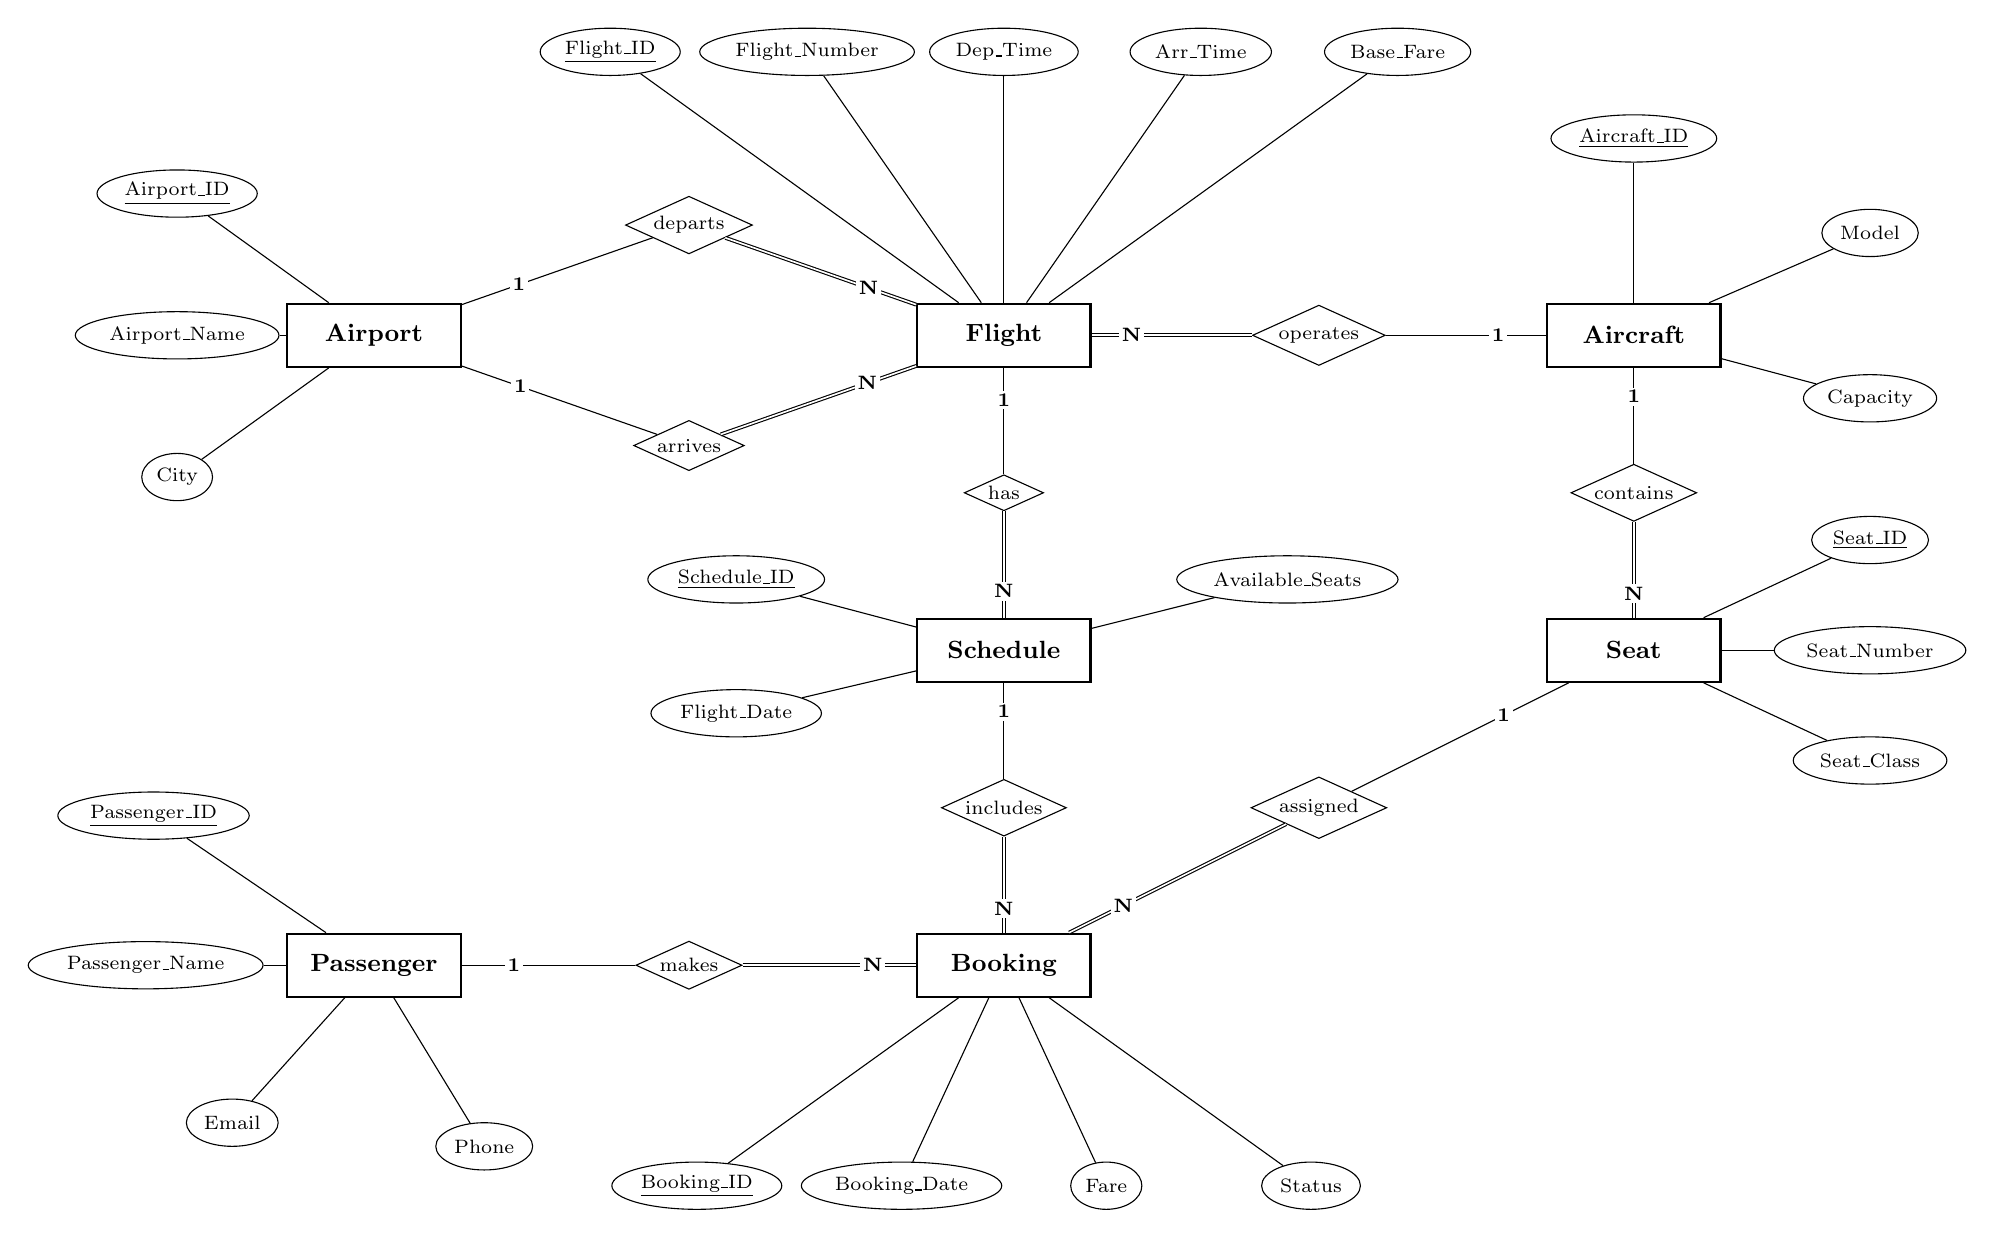
\begin{tikzpicture}[
  ent/.style={draw,rectangle,minimum width=2.2cm,minimum height=0.8cm,font=\small\bfseries,fill=white,line width=0.8pt},
  rel/.style={draw,diamond,aspect=2.2,inner sep=1pt,font=\scriptsize,fill=white},
  att/.style={draw,ellipse,font=\scriptsize,inner sep=1.5pt,minimum height=0.6cm,fill=white},
  card/.style={font=\scriptsize\bfseries,fill=white,inner sep=1pt},
  every double distance/.style={double distance=1.6pt}]
% entities
\node[ent] (Airport)   at (3,9)   {Airport};
\node[ent] (Flight)    at (11,9)  {Flight};
\node[ent] (Aircraft)  at (19,9)  {Aircraft};
\node[ent] (Schedule)  at (11,5)  {Schedule};
\node[ent] (Seat)      at (19,5)  {Seat};
\node[ent] (Passenger) at (3,1)   {Passenger};
\node[ent] (Booking)   at (11,1)  {Booking};
% relationships
\node[rel] (dep)  at (7,10.4)  {departs};
\node[rel] (arr)  at (7,7.6)   {arrives};
\node[rel] (op)   at (15,9)    {operates};
\node[rel] (has)  at (11,7)    {has};
\node[rel] (con)  at (19,7)    {contains};
\node[rel] (mk)   at (7,1)     {makes};
\node[rel] (inc)  at (11,3)    {includes};
\node[rel] (asg)  at (15,3)    {assigned};
% links
\draw (Airport) -- node[card,pos=.3]{1} (dep);
\draw[double] (dep) -- node[card,pos=.75]{N} (Flight);
\draw (Airport) -- node[card,pos=.3]{1} (arr);
\draw[double] (arr) -- node[card,pos=.75]{N} (Flight);
\draw (Aircraft) -- node[card,pos=.3]{1} (op);
\draw[double] (op) -- node[card,pos=.75]{N} (Flight);
\draw (Flight) -- node[card,pos=.3]{1} (has);
\draw[double] (has) -- node[card,pos=.75]{N} (Schedule);
\draw (Aircraft) -- node[card,pos=.3]{1} (con);
\draw[double] (con) -- node[card,pos=.75]{N} (Seat);
\draw (Passenger) -- node[card,pos=.3]{1} (mk);
\draw[double] (mk) -- node[card,pos=.75]{N} (Booking);
\draw (Schedule) -- node[card,pos=.3]{1} (inc);
\draw[double] (inc) -- node[card,pos=.75]{N} (Booking);
\draw (Seat) -- node[card,pos=.3]{1} (asg);
\draw[double] (asg) -- node[card,pos=.75]{N} (Booking);
% attribute macro
\newcommand{\attr}[4]{\node[att] (a#1) at (#2) {#3}; \draw (#4) -- (a#1);}
% Airport
\attr{1}{0.5,10.8}{\underline{Airport_ID}}{Airport}
\attr{2}{0.5,9}{Airport_Name}{Airport}
\attr{3}{0.5,7.2}{City}{Airport}
% Flight
\attr{4}{6,12.6}{\underline{Flight_ID}}{Flight}
\attr{5}{8.5,12.6}{Flight_Number}{Flight}
\attr{6}{11,12.6}{Dep_Time}{Flight}
\attr{7}{13.5,12.6}{Arr_Time}{Flight}
\attr{8}{16,12.6}{Base_Fare}{Flight}
% Aircraft
\attr{9}{19,11.5}{\underline{Aircraft_ID}}{Aircraft}
\attr{10}{22,10.3}{Model}{Aircraft}
\attr{11}{22,8.2}{Capacity}{Aircraft}
% Schedule
\attr{12}{7.6,5.9}{\underline{Schedule_ID}}{Schedule}
\attr{13}{7.6,4.2}{Flight_Date}{Schedule}
\attr{14}{14.6,5.9}{Available_Seats}{Schedule}
% Seat
\attr{15}{22,6.4}{\underline{Seat_ID}}{Seat}
\attr{16}{22,5}{Seat_Number}{Seat}
\attr{17}{22,3.6}{Seat_Class}{Seat}
% Passenger
\attr{18}{0.2,2.9}{\underline{Passenger_ID}}{Passenger}
\attr{19}{0.1,1}{Passenger_Name}{Passenger}
\attr{20}{1.2,-1}{Email}{Passenger}
\attr{21}{4.4,-1.3}{Phone}{Passenger}
% Booking
\attr{22}{7.1,-1.8}{\underline{Booking_ID}}{Booking}
\attr{23}{9.7,-1.8}{Booking_Date}{Booking}
\attr{24}{12.3,-1.8}{Fare}{Booking}
\attr{25}{14.9,-1.8}{Status}{Booking}
\end{tikzpicture}
\end{adjustbox}
\caption{ER Diagram of Airline Reservation System}
\end{figure}
\end{landscape}

% ================================================================
%                        4 RELATIONAL MODEL
% ================================================================
\section{Relational Model}
The relational model represents the data of the Airline Reservation System in the form of tables. The ER
model is converted using the standard mapping rules: every entity becomes a table whose key is its primary
key, and for every one-to-many relationship the primary key of the ``one'' side is placed as a foreign key
in the table on the ``many'' side.

\subsection{Relational Schema}
The relational tables used in the system are Airport, Aircraft, Flight, Schedule, Seat, Passenger, and
Booking, together with a supporting Booking_Audit table used by the audit trigger. Primary keys are
underlined and foreign keys are marked FK.
\begin{itemize}[nosep]
  \item \textbf{Airport}(\pk{Airport_ID}, Airport_Name, City)
  \item \textbf{Aircraft}(\pk{Aircraft_ID}, Model, Capacity)
  \item \textbf{Flight}(\pk{Flight_ID}, Flight_Number, \fk{Aircraft_ID}, \fk{Source_Airport}, \fk{Dest_Airport}, Dep_Time, Arr_Time, Base_Fare)
  \item \textbf{Schedule}(\pk{Schedule_ID}, \fk{Flight_ID}, Flight_Date, Available_Seats)
  \item \textbf{Seat}(\pk{Seat_ID}, \fk{Aircraft_ID}, Seat_Number, Seat_Class)
  \item \textbf{Passenger}(\pk{Passenger_ID}, Passenger_Name, Email, Phone)
  \item \textbf{Booking}(\pk{Booking_ID}, \fk{Passenger_ID}, \fk{Schedule_ID}, \fk{Seat_ID}, Booking_Date, Fare, Status)
  \item \textbf{Booking_Audit}(\pk{Audit_ID}, Booking_ID, Action_Type, Old_Status, New_Status, Changed_By, Changed_On)
\end{itemize}

\subsection{Primary Keys and Foreign Keys}
Each table has a primary key that uniquely identifies every record. Foreign keys connect related tables.
\begin{table}[H]
\centering\small
\begin{tabular}{l l l}
\toprule
\textbf{Table} & \textbf{Foreign key} & \textbf{References}\\
\midrule
Flight   & Aircraft_ID    & Aircraft(Aircraft_ID)\\
Flight   & Source_Airport & Airport(Airport_ID)\\
Flight   & Dest_Airport   & Airport(Airport_ID)\\
Schedule & Flight_ID      & Flight(Flight_ID)\\
Seat     & Aircraft_ID    & Aircraft(Aircraft_ID)\\
Booking  & Passenger_ID   & Passenger(Passenger_ID)\\
Booking  & Schedule_ID    & Schedule(Schedule_ID)\\
Booking  & Seat_ID        & Seat(Seat_ID)\\
\bottomrule
\end{tabular}
\caption{Foreign key constraints}
\end{table}
Besides the primary keys, the candidate keys Flight_Number, Email, Phone, and (Aircraft_ID, Seat_Number)
are declared UNIQUE.

% ================================================================
%                          5 NORMALIZATION
% ================================================================
\section{Normalization}
Normalization is the process of organizing data in a database to reduce redundancy and avoid insertion,
deletion, and update anomalies. The Airline Reservation System is normalized up to Third Normal Form (3NF)
and every determinant is also a candidate key, so the relations are in BCNF as well.

\subsection{Functional Dependencies}
The following functional dependencies are identified:
\begin{itemize}[nosep]
  \item Airport_ID $\rightarrow$ Airport_Name, City
  \item Aircraft_ID $\rightarrow$ Model, Capacity
  \item Flight_ID $\rightarrow$ Flight_Number, Aircraft_ID, Source_Airport, Dest_Airport, Dep_Time, Arr_Time, Base_Fare
  \item Flight_Number $\rightarrow$ Flight_ID \hfill (candidate key)
  \item Schedule_ID $\rightarrow$ Flight_ID, Flight_Date, Available_Seats
  \item Seat_ID $\rightarrow$ Aircraft_ID, Seat_Number, Seat_Class
  \item (Aircraft_ID, Seat_Number) $\rightarrow$ Seat_ID, Seat_Class \hfill (candidate key)
  \item Passenger_ID $\rightarrow$ Passenger_Name, Email, Phone
  \item Email $\rightarrow$ Passenger_ID; \quad Phone $\rightarrow$ Passenger_ID \hfill (candidate keys)
  \item Booking_ID $\rightarrow$ Passenger_ID, Schedule_ID, Seat_ID, Booking_Date, Fare, Status
\end{itemize}

\subsection{First Normal Form (1NF)}
A relation is in First Normal Form when all attributes contain atomic values and there are no repeating
groups. Suppose bookings were first recorded in a single sheet where one row holds several seats and a
passenger has several phone numbers:
\begin{table}[H]
\centering\small
\begin{tabular}{l l l l l}
\toprule
\textbf{Booking ID} & \textbf{Passenger} & \textbf{Phone} & \textbf{Flight} & \textbf{Seats}\\
\midrule
B1 & Ananya & 9876500001, 9876500011 & AI101 & 1A, 1B\\
B2 & Rohit  & 9876500002             & AI101 & 12C\\
\bottomrule
\end{tabular}
\caption{Unnormalized booking sheet (multi-valued attributes)}
\end{table}
To reach 1NF, each field is made atomic: the passenger is stored once in the Passenger relation and every
seat is stored in a separate Booking row, so one booking row stores exactly one seat.
\begin{table}[H]
\centering\small
\begin{tabular}{l l l l l r l}
\toprule
\textbf{Booking ID} & \textbf{Passenger ID} & \textbf{Schedule ID} & \textbf{Seat ID} & \textbf{Booking Date} & \textbf{Fare} & \textbf{Status}\\
\midrule
701 & 601 & 301 & 501 & 20-10-2026 & 9500 & Confirmed\\
702 & 602 & 301 & 502 & 21-10-2026 & 5500 & Confirmed\\
703 & 603 & 302 & 504 & 22-10-2026 & 4200 & Cancelled\\
\bottomrule
\end{tabular}
\caption{Booking relation in 1NF}
\end{table}

\subsection{Second Normal Form (2NF)}
A relation is in 2NF when it is in 1NF and every non-key attribute depends on the \emph{whole} primary key.
Consider a combined ticket relation with the composite key (Booking_ID, Seat_ID):
\[
\text{Ticket(\underline{Booking\_ID}, \underline{Seat\_ID}, Passenger\_Name, Fare, Seat\_Number, Seat\_Class)}
\]
Here Booking_ID $\rightarrow$ Passenger_Name, Fare and Seat_ID $\rightarrow$ Seat_Number, Seat_Class are
\emph{partial dependencies}, because the attributes depend on only a part of the key. They are removed by
placing booking details in Booking and seat details in Seat, so that Passenger_Name depends only on
Passenger_ID in Passenger, and Seat_Number and Seat_Class depend only on Seat_ID in Seat. In the final
design every relation has a single-attribute primary key, so no partial dependency can exist.

\subsection{Third Normal Form (3NF)}
A relation is in 3NF when it is in 2NF and has no transitive dependency between non-key attributes.
Consider a flight relation that also stores aircraft and airport details:
\[
\text{Flight\_Full(\underline{Flight\_ID}, Aircraft\_ID, Model, Capacity, Source\_Airport, Source\_City)}
\]
Here Flight_ID $\rightarrow$ Aircraft_ID and Aircraft_ID $\rightarrow$ Model, Capacity, so Model and Capacity
depend transitively on Flight_ID; likewise Flight_ID $\rightarrow$ Source_Airport $\rightarrow$ Source_City.
Repeating the model and city for every flight would cause update anomalies. They are removed by storing
only Aircraft_ID and the airport IDs in Flight, and keeping Model, Capacity, and City in the Aircraft and
Airport relations. Thus the final relations are:
\begin{itemize}[nosep]
  \item Airport(\pk{Airport_ID}, Airport_Name, City)
  \item Aircraft(\pk{Aircraft_ID}, Model, Capacity)
  \item Flight(\pk{Flight_ID}, Flight_Number, Aircraft_ID, Source_Airport, Dest_Airport, Dep_Time, Arr_Time, Base_Fare)
  \item Schedule(\pk{Schedule_ID}, Flight_ID, Flight_Date, Available_Seats)
  \item Seat(\pk{Seat_ID}, Aircraft_ID, Seat_Number, Seat_Class)
  \item Passenger(\pk{Passenger_ID}, Passenger_Name, Email, Phone)
  \item Booking(\pk{Booking_ID}, Passenger_ID, Schedule_ID, Seat_ID, Booking_Date, Fare, Status)
\end{itemize}
The database is therefore normalized up to 3NF, which reduces data redundancy and improves consistency
and maintainability.

% ================================================================
%                          6 SQL DDL
% ================================================================
\section{SQL DDL Commands}
Data Definition Language (DDL) commands create and modify the structure of database tables. In the Airline
Reservation System, DDL commands create the tables and define constraints such as primary keys, foreign
keys, UNIQUE, NOT NULL, and CHECK.

\subsection{Table Creation}
The following statements create the tables of the system. The complete script is available in
\texttt{sql/01\_ddl.sql}.
\sqlfile{01_ddl.sql}

\begin{figure}[H]
\begin{terminal}
SQL> @01_ddl.sql

Table created.   (Airport)
Table created.   (Aircraft)
Table created.   (Flight)
Table created.   (Schedule)
Table created.   (Seat)
Table created.   (Passenger)
Table created.   (Booking)

Index created.   (Uq_Active_Seat)

Table created.   (Booking_Audit)
\end{terminal}
\caption{Output of Table Creation}
\end{figure}

\subsection{Constraints}
\begin{table}[H]
\centering\small
\begin{tabularx}{\textwidth}{l X}
\toprule
\textbf{Constraint} & \textbf{Where used}\\
\midrule
PRIMARY KEY & Airport_ID, Aircraft_ID, Flight_ID, Schedule_ID, Seat_ID, Passenger_ID, Booking_ID, Audit_ID\\
FOREIGN KEY & Flight, Schedule, Seat, and Booking reference their parent tables (Table~3)\\
NOT NULL    & Airport_Name, City, Model, Flight_Number, Flight_Date, Seat_Number, Passenger_Name\\
UNIQUE      & Flight_Number, Email, Phone, (Aircraft_ID, Seat_Number)\\
CHECK       & Capacity $>$ 0, Base_Fare $>$ 0, Fare $>$ 0, Available_Seats $\ge$ 0, Seat_Class and Status in a fixed list, Source_Airport $\ne$ Dest_Airport\\
Unique index & Uq_Active_Seat: one \emph{confirmed} booking per seat per schedule\\
\bottomrule
\end{tabularx}
\caption{Summary of constraints}
\end{table}
Primary keys uniquely identify records and foreign keys establish relationships. NOT NULL ensures that
required fields contain values, UNIQUE prevents duplicates, and CHECK restricts values according to
specified conditions. The function-based unique index \texttt{Uq\_Active\_Seat} ignores cancelled bookings
(the indexed expressions are NULL for them), so a cancelled seat can be sold again while two confirmed
bookings for the same seat and schedule are impossible.

\subsection{ALTER Operation}
The ALTER command modifies an existing table: it can add a column, change a column definition, or add a
constraint.
\begin{code}
ALTER TABLE Passenger ADD Date_Of_Birth DATE;
ALTER TABLE Aircraft  MODIFY Model VARCHAR2(80);
ALTER TABLE Flight    ADD CONSTRAINT Chk_Flight_Times
      CHECK (Dep_Time <> Arr_Time);
\end{code}

\subsection{DROP Operation}
The DROP command removes a table and its stored records. It is demonstrated on a temporary copy so that the
real data is not lost.
\begin{code}
CREATE TABLE Flight_Archive AS SELECT * FROM Flight;
DROP TABLE Flight_Archive;
\end{code}

% ================================================================
%                          7 SQL DML
% ================================================================
\section{SQL DML Commands}
Data Manipulation Language (DML) commands insert, modify, and delete records. In the Airline Reservation
System they manage airport, flight, passenger, and booking information. The complete script is
\texttt{sql/02\_dml.sql}.

\subsection{INSERT}
The INSERT command adds new records to a table. The figure shows representative INSERT commands and their
output.
\begin{figure}[H]
\begin{terminal}
SQL> INSERT INTO Airport VALUES (101, 'Rajiv Gandhi International', 'Hyderabad');
1 row created.
SQL> INSERT INTO Aircraft VALUES (11, 'Airbus A320', 180);
1 row created.
SQL> INSERT INTO Flight VALUES (201, 'AI101', 11, 101, 102, '06:00', '08:10', 5500);
1 row created.
SQL> INSERT INTO Schedule VALUES (301, 201, TO_DATE('2026-11-15','YYYY-MM-DD'), 150);
1 row created.
SQL> INSERT INTO Seat VALUES (501, 11, '1A', 'Business');
1 row created.
SQL> INSERT INTO Passenger VALUES (601, 'Ananya', 'ananya@gmail.com', '9876500001');
1 row created.
SQL> INSERT INTO Booking VALUES (701, 601, 301, 501, TO_DATE('2026-10-20','YYYY-MM-DD'), 9500, 'Confirmed');
1 row created.
SQL> COMMIT;
Commit complete.
\end{terminal}
\caption{INSERT Commands and Output}
\end{figure}
The sample data set contains 4 airports, 2 aircraft, 3 flights, 3 schedules, 5 seats, 3 passengers, and
3 bookings.

\subsection{UPDATE}
The UPDATE command modifies existing records. For example, the status of a booking is changed when a
passenger cancels a ticket, and a contact number can be corrected.
\begin{code}
UPDATE Booking   SET Status = 'Cancelled' WHERE Booking_ID = 703;
UPDATE Passenger SET Phone = '9876500039' WHERE Passenger_ID = 603;
COMMIT;
\end{code}

\subsection{DELETE}
The DELETE command removes records. A passenger record that is not referenced by any booking can be
deleted, whereas deleting a passenger who has bookings is rejected by the foreign key.
\begin{code}
INSERT INTO Passenger VALUES (604, 'Kiran', 'kiran@gmail.com', '9876500004');
DELETE FROM Passenger WHERE Passenger_ID = 604;
COMMIT;
\end{code}
\begin{figure}[H]
\begin{terminal}
SQL> DELETE FROM Passenger WHERE Passenger_ID = 604;
1 row deleted.

SQL> DELETE FROM Passenger WHERE Passenger_ID = 601;
ERROR at line 1:
ORA-02292: integrity constraint violated - child record found
\end{terminal}
\caption{DELETE of an Unreferenced and a Referenced Passenger}
\end{figure}
DML commands help maintain and update the data stored in the database according to the operations
performed by passengers and administrators.

% ================================================================
%                          8 SQL QUERIES
% ================================================================
\section{SQL Queries}
SQL queries retrieve and analyze the data stored in the Airline Reservation System. The system uses SELECT
statements, joins, aggregate functions, subqueries, and views to obtain useful information.

\subsection{Basic SELECT Queries}
The SELECT command retrieves records from a table, with WHERE and ORDER BY used to filter and sort them.
\begin{figure}[H]
\begin{terminal}
SQL> SELECT Flight_ID, Flight_Number, Dep_Time, Arr_Time, Base_Fare FROM Flight;

 FLIGHT_ID FLIGHT_NUM DEP_TIME   ARR_TIME    BASE_FARE
---------- ---------- ---------- ---------- ----------
       201 AI101      06:00      08:10            5500
       202 6E202      09:30      11:00            4200
       203 UK303      14:00      16:45            6100

SQL> SELECT Airport_ID, City FROM Airport ORDER BY City;

AIRPORT_ID CITY
---------- --------------------
       104 Bengaluru
       102 Delhi
       101 Hyderabad
       103 Mumbai
\end{terminal}
\caption{Output of Basic SELECT Queries}
\end{figure}

\subsection{Joins}
Joins retrieve related information from two or more tables. The first query joins Flight, Schedule, and
Airport (twice) to show each dated flight with its route; the second joins Passenger and Booking; the third
is a LEFT OUTER JOIN that also lists flights without any booking.
\begin{figure}[H]
\begin{terminal}
SQL> SELECT F.Flight_Number, S.Flight_Date, A1.City AS Source, A2.City AS Destination
  2  FROM Flight F JOIN Schedule S ON F.Flight_ID = S.Flight_ID
  3  JOIN Airport A1 ON F.Source_Airport = A1.Airport_ID
  4  JOIN Airport A2 ON F.Dest_Airport   = A2.Airport_ID;

FLIGHT_NUMBER FLIGHT_DATE SOURCE          DESTINATION
------------- ----------- --------------- ---------------
AI101         15-NOV-26   Hyderabad       Delhi
6E202         16-NOV-26   Hyderabad       Mumbai
UK303         17-NOV-26   Delhi           Bengaluru

SQL> SELECT P.Passenger_Name, B.Booking_ID, B.Status
  2  FROM Passenger P JOIN Booking B ON P.Passenger_ID = B.Passenger_ID;

PASSENGER_NAME       BOOKING_ID STATUS
-------------------- ---------- ----------
Ananya                      701 Confirmed
Rohit                       702 Confirmed
Meera                       703 Cancelled

SQL> SELECT F.Flight_Number, COUNT(B.Booking_ID) AS Bookings
  2  FROM Flight F LEFT JOIN Schedule S ON F.Flight_ID = S.Flight_ID
  3  LEFT JOIN Booking B ON S.Schedule_ID = B.Schedule_ID
  4  GROUP BY F.Flight_Number ORDER BY F.Flight_Number;

FLIGHT_NUMBER  BOOKINGS
------------- ---------
6E202                 1
AI101                 2
UK303                 0
\end{terminal}
\caption{Output of Join Queries}
\end{figure}

\subsection{Aggregate Functions}
Aggregate functions such as COUNT, SUM, AVG, MAX, and MIN perform calculations on records.
\begin{figure}[H]
\begin{terminal}
SQL> SELECT COUNT(*) AS Total_Bookings FROM Booking;

TOTAL_BOOKINGS
--------------
             3

SQL> SELECT SUM(Fare) AS Confirmed_Revenue FROM Booking WHERE Status = 'Confirmed';

CONFIRMED_REVENUE
-----------------
            15000

SQL> SELECT ROUND(AVG(Base_Fare),2) AS Avg_Fare, MAX(Base_Fare) AS Highest,
  2         MIN(Base_Fare) AS Lowest FROM Flight;

  AVG_FARE    HIGHEST     LOWEST
---------- ---------- ----------
   5266.67       6100       4200
\end{terminal}
\caption{Output of Aggregate Functions}
\end{figure}

\subsection{GROUP BY and HAVING}
GROUP BY groups records, while HAVING applies conditions to the groups.
\begin{figure}[H]
\begin{terminal}
SQL> SELECT Status, COUNT(*) AS Total FROM Booking GROUP BY Status ORDER BY Status;

STATUS                   TOTAL
-------------------- ----------
Cancelled                     1
Confirmed                     2

SQL> SELECT Status, COUNT(*) AS Total FROM Booking
  2  GROUP BY Status HAVING COUNT(*) > 1;

STATUS                   TOTAL
-------------------- ----------
Confirmed                     2

SQL> SELECT Schedule_ID, SUM(Fare) AS Revenue FROM Booking
  2  WHERE Status = 'Confirmed' GROUP BY Schedule_ID HAVING SUM(Fare) > 10000;

SCHEDULE_ID    REVENUE
----------- ----------
        301      15000
\end{terminal}
\caption{Output of GROUP BY and HAVING Queries}
\end{figure}

\subsection{Subqueries}
A subquery is a query written inside another query. The first query lists flights whose base fare is above
the average; the second is a nested query (four levels) that finds passengers with a confirmed booking on a
flight departing from Hyderabad; the third is a correlated subquery using EXISTS.
\begin{figure}[H]
\begin{terminal}
SQL> SELECT Flight_Number, Base_Fare FROM Flight
  2  WHERE Base_Fare > (SELECT AVG(Base_Fare) FROM Flight);

FLIGHT_NUMBER   BASE_FARE
------------- -----------
AI101                5500
UK303                6100

SQL> SELECT Passenger_Name FROM Passenger WHERE Passenger_ID IN
  2   (SELECT Passenger_ID FROM Booking WHERE Status = 'Confirmed' AND Schedule_ID IN
  3     (SELECT Schedule_ID FROM Schedule WHERE Flight_ID IN
  4       (SELECT Flight_ID FROM Flight WHERE Source_Airport =
  5         (SELECT Airport_ID FROM Airport WHERE City = 'Hyderabad'))));

PASSENGER_NAME
--------------------
Ananya
Rohit

SQL> SELECT Passenger_Name FROM Passenger P WHERE EXISTS
  2   (SELECT 1 FROM Booking B WHERE B.Passenger_ID = P.Passenger_ID
  3      AND B.Status = 'Cancelled');

PASSENGER_NAME
--------------------
Meera
\end{terminal}
\caption{Output of Subqueries}
\end{figure}

\subsection{Views}
A view is a virtual table created from the result of an SQL query. The view \texttt{Booking\_Details}
hides the five-table join and is reused by the reports in Section~13.
\begin{figure}[H]
\begin{terminal}
SQL> CREATE VIEW Booking_Details AS
  2  SELECT B.Booking_ID, P.Passenger_Name, F.Flight_Number, S.Flight_Date,
  3         St.Seat_Number, B.Fare, B.Status
  4  FROM Booking B JOIN Passenger P ON B.Passenger_ID = P.Passenger_ID
  5  JOIN Schedule S ON B.Schedule_ID = S.Schedule_ID
  6  JOIN Flight F   ON S.Flight_ID   = F.Flight_ID
  7  JOIN Seat St    ON B.Seat_ID     = St.Seat_ID;

View created.

SQL> SELECT * FROM Booking_Details;

BOOKING_ID PASSENGER_NAME  FLIGHT_NUMBER FLIGHT_DATE SEAT_NUMBER  FARE STATUS
---------- --------------- ------------- ----------- ----------- ----- ----------
       701 Ananya          AI101         15-NOV-26   1A           9500 Confirmed
       702 Rohit           AI101         15-NOV-26   12C          5500 Confirmed
       703 Meera           6E202         16-NOV-26   5A           4200 Cancelled
\end{terminal}
\caption{Creation and Output of Booking Details View}
\end{figure}

% ================================================================
%                  9 TRANSACTIONS AND CONCURRENCY
% ================================================================
\section{Transactions and Concurrency}
Transactions are a sequence of database operations performed as a single logical unit. In the Airline
Reservation System, transactions ensure that booking and cancellation operations are completed correctly and
consistently.

\subsection{Transaction Management}
A transaction begins with the first DML statement and ends when the changes are either permanently saved or
cancelled. Booking a ticket involves checking the seat, creating the booking, and reducing the available
seat count; either all of these steps happen or none of them do (atomicity).

\subsection{COMMIT, ROLLBACK and SAVEPOINT}
COMMIT permanently saves the changes made by a transaction. ROLLBACK cancels the changes made since the
beginning of the transaction or since the last SAVEPOINT. SAVEPOINT creates a point within a transaction
to which the transaction can be partially rolled back. The script is \texttt{sql/09\_transactions.sql}.
\begin{figure}[H]
\begin{terminal}
SQL> INSERT INTO Booking VALUES (704, 601, 302, 505, TO_DATE('2026-10-25','YYYY-MM-DD'), 4200, 'Confirmed');
1 row created.

SQL> SAVEPOINT booking_save;
Savepoint created.

SQL> UPDATE Booking SET Status = 'Cancelled' WHERE Booking_ID = 704;
1 row updated.

SQL> ROLLBACK TO booking_save;
Rollback complete.

SQL> SELECT Booking_ID, Status FROM Booking WHERE Booking_ID = 704;

BOOKING_ID STATUS
---------- ----------
       704 Confirmed

SQL> ROLLBACK;
Rollback complete.

SQL> SELECT COUNT(*) FROM Booking WHERE Booking_ID = 704;

  COUNT(*)
----------
         0

SQL> UPDATE Passenger SET Email = 'ananya.s@gmail.com' WHERE Passenger_ID = 601;
1 row updated.

SQL> COMMIT;
Commit complete.

SQL> ROLLBACK;
Rollback complete.

SQL> SELECT Email FROM Passenger WHERE Passenger_ID = 601;

EMAIL
--------------------
ananya.s@gmail.com
\end{terminal}
\caption{Output of COMMIT, ROLLBACK and SAVEPOINT Operations}
\end{figure}
The first block shows that ROLLBACK TO \texttt{booking\_save} undoes only the cancellation, keeping the
INSERT, while the full ROLLBACK removes the booking completely. The second block shows that once a change is
COMMITted it is permanent, so the later ROLLBACK has no effect.

\subsection{Concurrency Control}
Concurrency control manages simultaneous transactions that access the same data. In an airline system many
passengers try to book the last seats of a popular flight at the same moment.

\paragraph{The problem.} Suppose two passengers, in Session A and Session B, both want seat 12D on flight
AI101 (Schedule 301). Each session first checks that the seat has no confirmed booking and then inserts a
booking. Without protection both checks return 0 before either insert happens, so \emph{both} inserts
succeed and the seat is sold twice (a lost-update / double-booking anomaly). The same interleaving applied
to \texttt{Available\_Seats} (both read 150 and both write 149) would lose one update.

\paragraph{The solution.} A session locks the schedule row with \texttt{SELECT ... FOR UPDATE} before it
checks and books. A second session asking for the same lock must wait until the first one ends with COMMIT
or ROLLBACK; afterwards its check sees the committed booking and the request is rejected. The
\texttt{Book\_Ticket} procedure (Section~10.2) uses the same technique, and the unique index
\texttt{Uq\_Active\_Seat} acts as a final safety net. Seat counts are changed with
\texttt{Available\_Seats = Available\_Seats - 1}, which is atomic under the row lock.
\begin{table}[H]
\centering\small
\begin{tabularx}{\textwidth}{l X X}
\toprule
\textbf{Time} & \textbf{Session A} & \textbf{Session B}\\
\midrule
T1 & Locks Schedule 301 (\texttt{FOR UPDATE}) & \\
T2 &  & Requests the same lock --- \emph{waits}\\
T3 & Checks seat 503: 0 confirmed bookings; inserts Booking 704 & (still waiting)\\
T4 & \texttt{COMMIT} --- lock released & \\
T5 &  & Lock granted; check finds 1 confirmed booking\\
T6 &  & Booking rejected, \texttt{ROLLBACK}\\
\bottomrule
\end{tabularx}
\caption{Timeline of two concurrent booking transactions}
\end{table}
\begin{figure}[H]
\begin{terminal}
-- ---------------------------- SESSION A ----------------------------
SQL> SELECT Schedule_ID, Available_Seats FROM Schedule WHERE Schedule_ID = 301 FOR UPDATE;

SCHEDULE_ID AVAILABLE_SEATS
----------- ---------------
        301             150

SQL> SELECT COUNT(*) FROM Booking
  2  WHERE Schedule_ID = 301 AND Seat_ID = 503 AND Status = 'Confirmed';

  COUNT(*)
----------
         0

SQL> INSERT INTO Booking VALUES (704, 601, 301, 503, SYSDATE, 5500, 'Confirmed');
1 row created.

SQL> COMMIT;
Commit complete.

-- ---------------------------- SESSION B ----------------------------
SQL> SELECT Schedule_ID, Available_Seats FROM Schedule WHERE Schedule_ID = 301 FOR UPDATE;
        (session waits until Session A commits ...)

SCHEDULE_ID AVAILABLE_SEATS
----------- ---------------
        301             149

SQL> SELECT COUNT(*) FROM Booking
  2  WHERE Schedule_ID = 301 AND Seat_ID = 503 AND Status = 'Confirmed';

  COUNT(*)
----------
         1

Seat 12D is already booked - request rejected.
SQL> ROLLBACK;
Rollback complete.
\end{terminal}
\caption{Concurrent Booking Scenario: Locking Prevents Double Booking}
\end{figure}
If a session skips the lock and inserts anyway, the database still protects the data:
\begin{figure}[H]
\begin{terminal}
SQL> INSERT INTO Booking VALUES (705, 602, 301, 503, SYSDATE, 5500, 'Confirmed');
ERROR at line 1:
ORA-00001: unique constraint (UQ_ACTIVE_SEAT) violated
\end{terminal}
\caption{Unique Index as Safety Net Against Duplicate Seat Reservation}
\end{figure}
Test data from this demonstration is removed afterwards with \texttt{DELETE FROM Booking WHERE Booking\_ID
= 704; COMMIT;}. Thus, transaction management and concurrency control ensure reliable and consistent
ticket reservations.

% ================================================================
%                         10 PL/SQL
% ================================================================
\section{PL/SQL Implementation}
PL/SQL is a procedural extension of SQL that allows programming constructs such as variables, conditions,
loops, procedures, functions, cursors, and triggers. In the Airline Reservation System, PL/SQL implements
the business operations and automates repetitive tasks.

\subsection{Functions}
A function is a stored PL/SQL program that accepts parameters and returns a value. Two functions are
implemented: \texttt{Get\_Booking\_Count} returns the number of bookings of a passenger, and
\texttt{Calculate\_Refund} returns the refund for a cancelled booking (80\% of the fare, 0 otherwise, and
$-1$ for an invalid booking).
\sqlfile{04_functions.sql}
\begin{figure}[H]
\begin{terminal}
SQL> SELECT Get_Booking_Count(601) AS Bookings FROM DUAL;

  BOOKINGS
----------
         1

SQL> SELECT Calculate_Refund(703) AS Refund FROM DUAL;

    REFUND
----------
      3360

SQL> SELECT Calculate_Refund(999) AS Refund FROM DUAL;

    REFUND
----------
        -1
\end{terminal}
\caption{Output of PL/SQL Functions}
\end{figure}

\subsection{Stored Procedures}
A stored procedure is a named PL/SQL program that performs a major business operation.
\texttt{Book\_Ticket} validates the request, locks the schedule, rejects unavailable or invalid seats, and
creates the booking; \texttt{Cancel\_Booking} cancels a booking and reports the refund.
\sqlfile{05_procedures.sql}
\begin{figure}[H]
\begin{terminal}
SQL> SET SERVEROUTPUT ON
SQL> EXEC Book_Ticket(602, 303, 503, 6100);
Booking confirmed. Booking ID: 704

SQL> EXEC Book_Ticket(602, 301, 502, 5500);
ERROR at line 1:
ORA-20002: Seat already booked

SQL> EXEC Book_Ticket(602, 302, 503, 4200);
ERROR at line 1:
ORA-20004: Seat does not belong to this flight

SQL> EXEC Cancel_Booking(704);
Booking cancelled. Refund: Rs. 4880

SQL> EXEC Cancel_Booking(704);
ERROR at line 1:
ORA-20005: Booking already cancelled

SQL> DELETE FROM Booking WHERE Booking_ID = 704;   -- remove test data
SQL> COMMIT;
\end{terminal}
\caption{Execution of Stored Procedures}
\end{figure}

\subsection{Cursors}
A cursor processes the rows returned by a query one at a time. An \emph{explicit cursor} prepares the
revenue report of every flight, and the \emph{implicit cursor} attribute \texttt{SQL\%ROWCOUNT} reports how
many bookings a batch cancellation (for example when a flight is called off) affected.
\sqlfile{06_cursors.sql}
\begin{figure}[H]
\begin{terminal}
6E202     Rs. 0
AI101     Rs. 15000
UK303     Rs. 0

PL/SQL procedure successfully completed.

SQL> EXEC Cancel_Schedule(303);
0 booking(s) cancelled.
\end{terminal}
\caption{Output of the Explicit and Implicit Cursors}
\end{figure}

\subsection{Triggers}
A trigger is a PL/SQL program that executes automatically when a specified database event occurs. Three
triggers are defined on Booking: \texttt{Booking\_Validate} sets defaults and rejects bookings made after
the flight date, \texttt{Seat\_Inventory} keeps \texttt{Schedule.Available\_Seats} up to date, and
\texttt{Booking\_Audit\_Trg} records the history of every change in \texttt{Booking\_Audit}.
\sqlfile{07_triggers.sql}
\begin{figure}[H]
\begin{terminal}
SQL> INSERT INTO Booking (Booking_ID, Passenger_ID, Schedule_ID, Seat_ID, Fare)
  2  VALUES (705, 601, 302, 505, 4200);
1 row created.

SQL> SELECT Booking_ID, Status FROM Booking WHERE Booking_ID = 705;

BOOKING_ID STATUS
---------- ----------
       705 Confirmed

SQL> SELECT Schedule_ID, Available_Seats FROM Schedule WHERE Schedule_ID = 302;

SCHEDULE_ID AVAILABLE_SEATS
----------- ---------------
        302             119

SQL> SELECT Booking_ID, Action_Type, Old_Status, New_Status
  2  FROM Booking_Audit WHERE Booking_ID = 705;

BOOKING_ID ACTION_TYP OLD_STATUS NEW_STATUS
---------- ---------- ---------- ----------
       705 INSERT                Confirmed

SQL> INSERT INTO Booking (Booking_ID, Passenger_ID, Schedule_ID, Seat_ID, Booking_Date, Fare)
  2  VALUES (706, 602, 302, 504, TO_DATE('2026-11-20','YYYY-MM-DD'), 4200);
ERROR at line 1:
ORA-20010: Cannot book a flight that has already departed

SQL> ROLLBACK;
Rollback complete.
\end{terminal}
\caption{Output of Trigger Execution}
\end{figure}
The first insert omits the status and date, which the trigger fills in; the seat count falls from 120 to
119 and an audit row is written. The second insert is rejected by the validation trigger. The final
ROLLBACK undoes the test data. PL/SQL functions, procedures, cursors, and triggers improve automation,
reduce repeated operations, and help maintain consistency in the database.

% ================================================================
%                11 FILE ORGANIZATION AND INDEXING
% ================================================================
\section{File Organization and Indexing}
File organization defines how records are stored and arranged in a database file. Indexing improves the
speed of data retrieval by providing an efficient way to locate records. In the Airline Reservation System
the most frequently searched attributes are Flight_ID, Schedule_ID, Seat_ID, Passenger_ID, and Booking_ID.

\subsection{File Organization}
\begin{table}[H]
\centering\small
\begin{tabularx}{\textwidth}{l X X}
\toprule
\textbf{Organization} & \textbf{How records are stored} & \textbf{Use in this project}\\
\midrule
Sequential & Records kept in order of a key; good for full scans and reports & Flight records ordered by Flight_ID for the daily flight listing\\
Heap       & Records appended wherever space is free; fast inserts, slow searches & Default Oracle table storage; used for Booking, where new rows arrive continuously\\
Indexed    & Records located through an index on a key & Index-organized table and B+ tree indexes for Booking_ID, Passenger_ID, and Flight_ID lookups\\
\bottomrule
\end{tabularx}
\caption{File organizations considered}
\end{table}
Oracle stores ordinary tables as heaps, so sequential retrieval is obtained with ORDER BY. Indexed file
organization is demonstrated with an index-organized table, whose rows are stored inside the primary-key
B+ tree itself:
\begin{code}
CREATE TABLE Booking_IOT (
    Booking_ID  INT PRIMARY KEY,
    Schedule_ID INT,
    Fare        NUMBER(10,2)
) ORGANIZATION INDEX;
\end{code}

\subsection{ISAM}
Indexed Sequential Access Method (ISAM) stores records sequentially in primary data pages and keeps a
\emph{static} index over them. It supports both sequential and direct access. The index is built once; when
a data page becomes full, new records are chained to an \emph{overflow page}, so the structure degrades if
many records are inserted. Figure~\ref{fig:isam} shows an ISAM file on Seat_ID (page capacity two keys)
after Seat_ID 507 is inserted into the full page holding 505 and 506. A search for Seat_ID 507 reads the
index page, follows the pointer to the third data page, and then follows its overflow chain.
\begin{figure}[H]
\centering
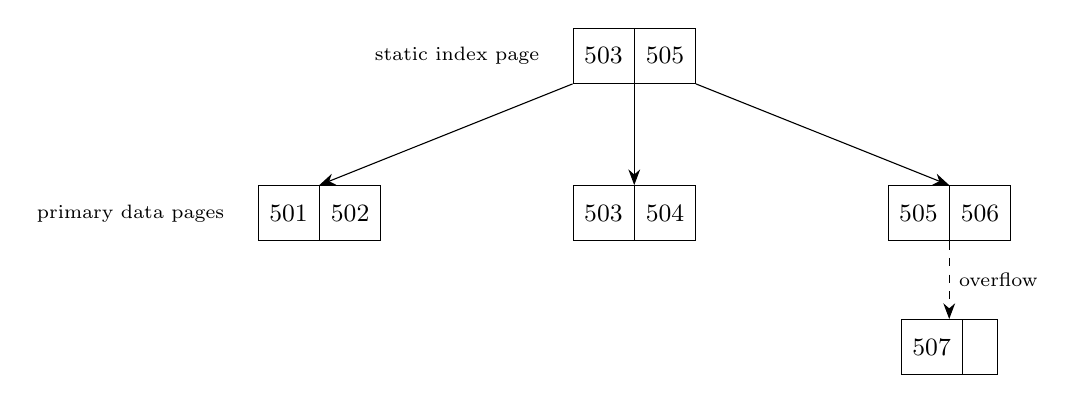
\begin{tikzpicture}[
  bn/.style={draw,rectangle split,rectangle split horizontal,rectangle split parts=2,minimum height=0.7cm,inner sep=4pt,font=\small},
  >={Stealth[length=2mm]}]
\node[bn] (I)  at (0,0)   {503\nodepart{two}505};
\node[bn] (P1) at (-4,-2) {501\nodepart{two}502};
\node[bn] (P2) at (0,-2)  {503\nodepart{two}504};
\node[bn] (P3) at (4,-2)  {505\nodepart{two}506};
\node[bn] (O1) at (4,-3.7) {507\nodepart{two}~};
\draw[->] (I.south west) -- (P1.north);
\draw[->] (I.south)      -- (P2.north);
\draw[->] (I.south east) -- (P3.north);
\draw[->,dashed] (P3.south) -- node[right,font=\scriptsize]{overflow} (O1.north);
\node[font=\scriptsize,left=0.3cm of I] {static index page};
\node[font=\scriptsize,left=0.3cm of P1] {primary data pages};
\end{tikzpicture}
\caption{ISAM Structure on Seat\_ID with an Overflow Page}\label{fig:isam}
\end{figure}

\subsection{B+ Tree Indexing}
A B+ tree is a balanced tree structure commonly used for database indexing. Internal nodes hold only index
keys, the leaf nodes hold the keys with record pointers, and the leaves are linked, which makes sequential
and range searches efficient. Unlike ISAM, a B+ tree splits nodes as it grows and therefore stays balanced
without overflow chains. Oracle's default index is a B+ tree. Figure~\ref{fig:bplus} shows a B+ tree on
Seat_ID.
\begin{figure}[H]
\centering
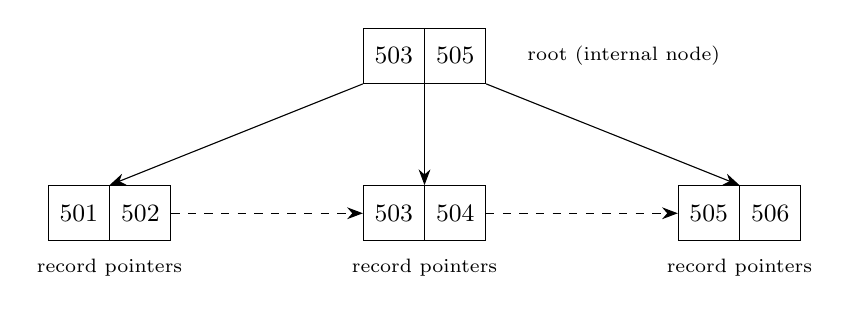
\begin{tikzpicture}[
  bn/.style={draw,rectangle split,rectangle split horizontal,rectangle split parts=2,minimum height=0.7cm,inner sep=4pt,font=\small},
  >={Stealth[length=2mm]}]
\node[bn] (R)  at (0,0)   {503\nodepart{two}505};
\node[bn] (L1) at (-4,-2) {501\nodepart{two}502};
\node[bn] (L2) at (0,-2)  {503\nodepart{two}504};
\node[bn] (L3) at (4,-2)  {505\nodepart{two}506};
\draw[->] (R.south west) -- (L1.north);
\draw[->] (R.south)      -- (L2.north);
\draw[->] (R.south east) -- (L3.north);
\draw[->,dashed] (L1.east) -- (L2.west);
\draw[->,dashed] (L2.east) -- (L3.west);
\node[font=\scriptsize,below=0.1cm of L1] {record pointers};
\node[font=\scriptsize,below=0.1cm of L2] {record pointers};
\node[font=\scriptsize,below=0.1cm of L3] {record pointers};
\node[font=\scriptsize,right=0.4cm of R] {root (internal node)};
\end{tikzpicture}
\caption{B+ Tree Index on Seat\_ID (dashed arrows: linked leaf nodes)}\label{fig:bplus}
\end{figure}
The primary keys are indexed automatically. The following secondary indexes speed up the most common
searches (script \texttt{sql/08\_indexes.sql}):
\begin{code}
CREATE INDEX Idx_Booking_Passenger ON Booking(Passenger_ID);
CREATE INDEX Idx_Schedule_Flight   ON Schedule(Flight_ID);
CREATE INDEX Idx_Flight_Route      ON Flight(Source_Airport, Dest_Airport);
\end{code}
The effect is visible in the execution plan. On a table with only a few rows the optimizer may still choose
a full table scan; with a large number of bookings the index is used, as shown below.
\begin{figure}[H]
\begin{terminal}
SQL> EXPLAIN PLAN FOR SELECT * FROM Booking WHERE Passenger_ID = 602;
Explained.

SQL> SELECT * FROM TABLE(DBMS_XPLAN.DISPLAY);

-----------------------------------------------------------------------------------
| Id | Operation                           | Name                  | Rows | Cost |
-----------------------------------------------------------------------------------
|  0 | SELECT STATEMENT                    |                       |    1 |    2 |
|  1 |  TABLE ACCESS BY INDEX ROWID BATCHED| BOOKING               |    1 |    2 |
|* 2 |   INDEX RANGE SCAN                  | IDX_BOOKING_PASSENGER |    1 |    1 |
-----------------------------------------------------------------------------------
Predicate Information (identified by operation id):
   2 - access("PASSENGER_ID"=602)
\end{terminal}
\caption{Execution Plan Using the B+ Tree Index}
\end{figure}
B+ tree indexing improves search performance and reduces the number of database blocks that must be
accessed. It is especially useful when the database contains a large number of flight, schedule, and
booking records.

% ================================================================
%                            12 TESTING
% ================================================================
\section{Testing}
Testing verifies that the Airline Reservation System works correctly and produces the expected results.
Test cases cover normal operations, boundary conditions, invalid inputs, and transaction and concurrency
behaviour.

\subsection{Test Cases}
The following test cases verify the main functions of the system.
\begin{table}[H]
\centering\small
\begin{tabularx}{\textwidth}{l l X l}
\toprule
\textbf{Test ID} & \textbf{Test case} & \textbf{Expected result} & \textbf{Status}\\
\midrule
TC01 & Search flights Hyderabad to Delhi & Flight AI101 on 15-NOV-26 is displayed & Pass\\
TC02 & Book an available seat with \texttt{Book\_Ticket} & Booking created with status Confirmed; Available_Seats reduced by 1 & Pass\\
TC03 & Cancel a valid booking & Status becomes Cancelled; seat count restored; refund = 80\% of fare & Pass\\
TC04 & View all bookings through \texttt{Booking\_Details} & All bookings with passenger and flight names are listed & Pass\\
TC05 & Run the revenue report & Revenue equals the sum of confirmed fares (15000 for AI101) & Pass\\
\bottomrule
\end{tabularx}
\caption{Functional test cases}
\end{table}

\subsection{Normal and Boundary Cases}
Normal cases use valid inputs, such as selecting an available seat and entering valid passenger details.
Boundary cases test values at the limits.
\begin{table}[H]
\centering\small
\begin{tabularx}{\textwidth}{l X X l}
\toprule
\textbf{Test ID} & \textbf{Boundary case} & \textbf{Expected result} & \textbf{Status}\\
\midrule
TC06 & Book the last seat (Available_Seats = 1) & Booking succeeds; Available_Seats becomes 0 & Pass\\
TC07 & Book when Available_Seats = 0 & Rejected with ORA-20001 (No seats available) & Pass\\
TC08 & Insert aircraft with Capacity = 1 and Capacity = 0 & 1 accepted; 0 rejected by CHECK (ORA-02290) & Pass\\
TC09 & Booking_Date equal to Flight_Date / one day after & Same day accepted; next day rejected (ORA-20010) & Pass\\
TC10 & First seat (1A) and last seat of an aircraft & Both can be booked normally & Pass\\
\bottomrule
\end{tabularx}
\caption{Normal and boundary test cases}
\end{table}

\subsection{Invalid Input Testing}
Invalid input testing verifies that incorrect data is rejected and database consistency is maintained.
\begin{table}[H]
\centering\small
\begin{tabularx}{\textwidth}{l X X l}
\toprule
\textbf{Test ID} & \textbf{Invalid input} & \textbf{Expected result} & \textbf{Status}\\
\midrule
TC11 & Booking for a non-existing passenger ID & ORA-02291 parent key not found & Pass\\
TC12 & Booking Status = 'Pending' & ORA-02290 CHECK constraint violated & Pass\\
TC13 & Passenger with an existing e-mail & ORA-00001 unique constraint violated & Pass\\
TC14 & Flight with Source_Airport = Dest_Airport & ORA-02290 CHECK constraint violated & Pass\\
TC15 & Negative or zero fare & ORA-02290 CHECK constraint violated & Pass\\
TC16 & Delete a passenger who has bookings & ORA-02292 child record found & Pass\\
TC17 & Cancel an already cancelled booking & ORA-20005 Booking already cancelled & Pass\\
TC18 & Book a seat of another aircraft & ORA-20004 Seat does not belong to this flight & Pass\\
\bottomrule
\end{tabularx}
\caption{Invalid input test cases}
\end{table}

\subsection{Transaction and Concurrency Testing}
\begin{table}[H]
\centering\small
\begin{tabularx}{\textwidth}{l X X l}
\toprule
\textbf{Test ID} & \textbf{Scenario} & \textbf{Expected result} & \textbf{Status}\\
\midrule
TC19 & Insert a booking, then ROLLBACK & Booking does not exist afterwards & Pass\\
TC20 & Change a booking, SAVEPOINT, change again, ROLLBACK TO savepoint & Only the second change is undone & Pass\\
TC21 & COMMIT followed by ROLLBACK & Committed change remains & Pass\\
TC22 & Two sessions book the same seat at the same time & Second session waits, then is rejected; one confirmed booking only & Pass\\
TC23 & Two sessions book different seats on the same flight & Both succeed; Available_Seats reduced by exactly 2 & Pass\\
TC24 & Booking inserted without locking while seat is taken & ORA-00001 from Uq_Active_Seat & Pass\\
\bottomrule
\end{tabularx}
\caption{Transaction and concurrency test cases}
\end{table}
Testing ensures that the system performs its operations correctly and helps identify errors before the
system is used in practice.

% ================================================================
%                             13 REPORTS
% ================================================================
\section{Reports}
The Airline Reservation System generates reports that provide useful information about ticket bookings,
cancellations, and revenue. These reports help administrators monitor the activities of the system and make
better decisions. All reports are produced with SQL queries over the data set of Section~7.

\subsection{Booking Report}
The booking report lists the tickets booked by passengers with flight, seat, fare, and status.
\begin{code}
SELECT Booking_ID, Passenger_Name, Flight_Number, Seat_Number, Fare, Status
FROM Booking_Details ORDER BY Booking_ID;
\end{code}
\begin{table}[H]
\centering\small
\begin{tabular}{l l l l r l}
\toprule
\textbf{Booking ID} & \textbf{Passenger} & \textbf{Flight} & \textbf{Seat} & \textbf{Fare} & \textbf{Status}\\
\midrule
701 & Ananya & AI101 & 1A  & Rs. 9500 & Confirmed\\
702 & Rohit  & AI101 & 12C & Rs. 5500 & Confirmed\\
703 & Meera  & 6E202 & 5A  & Rs. 4200 & Cancelled\\
\bottomrule
\end{tabular}
\caption{Sample Booking Report}
\end{table}

\subsection{Cancellation Report}
The cancellation report displays the cancelled bookings and the refund payable, helping administrators
track cancelled tickets.
\begin{code}
SELECT B.Booking_ID, P.Passenger_Name, B.Booking_Date, B.Fare,
       Calculate_Refund(B.Booking_ID) AS Refund
FROM Booking B JOIN Passenger P ON B.Passenger_ID = P.Passenger_ID
WHERE B.Status = 'Cancelled';
\end{code}
\begin{table}[H]
\centering\small
\begin{tabular}{l l l r r}
\toprule
\textbf{Booking ID} & \textbf{Passenger} & \textbf{Booking Date} & \textbf{Fare} & \textbf{Refund}\\
\midrule
703 & Meera & 2026-10-22 & Rs. 4200 & Rs. 3360\\
\bottomrule
\end{tabular}
\caption{Sample Cancellation Report}
\end{table}

\subsection{Revenue Report}
The revenue report gives the income generated from confirmed bookings for every dated flight, so that
administrators can analyze the financial performance of each route.
\begin{code}
SELECT F.Flight_Number, S.Flight_Date,
       COUNT(CASE WHEN B.Status = 'Confirmed' THEN 1 END) AS Tickets,
       NVL(SUM(CASE WHEN B.Status = 'Confirmed' THEN B.Fare END), 0) AS Revenue
FROM Flight F JOIN Schedule S ON S.Flight_ID = F.Flight_ID
LEFT JOIN Booking B ON B.Schedule_ID = S.Schedule_ID
GROUP BY F.Flight_Number, S.Flight_Date
ORDER BY S.Flight_Date;
\end{code}
\begin{table}[H]
\centering\small
\begin{tabular}{l l r r}
\toprule
\textbf{Flight} & \textbf{Flight Date} & \textbf{Tickets} & \textbf{Revenue}\\
\midrule
AI101 & 2026-11-15 & 2 & Rs. 15000\\
6E202 & 2026-11-16 & 0 & Rs. 0\\
UK303 & 2026-11-17 & 0 & Rs. 0\\
\bottomrule
\end{tabular}
\caption{Sample Revenue Report}
\end{table}
The same revenue figures are produced by the cursor-based procedure of Section~10.3. These reports provide a
clear summary of booking activities, cancellations, and revenue, helping administrators manage the airline
reservation system efficiently.

% ================================================================
%                     14 RESULTS AND DISCUSSION
% ================================================================
\section{Results and Discussion}
The Airline Reservation System successfully provides a structured database for managing airports, aircraft,
flights, schedules, seats, passengers, and bookings. The implemented SQL commands allow records to be
created, updated, deleted, and retrieved efficiently.

The database design reduces data redundancy through normalization up to 3NF and maintains data integrity
using primary keys, foreign keys, UNIQUE, NOT NULL, and CHECK constraints. Transactions and locking prevent
the same seat from being sold twice when several passengers book at the same time, and the unique index on
confirmed bookings guarantees this even if the application code is bypassed.

The implemented PL/SQL functions, procedures, cursors, and triggers provide additional automation: seat
counts are updated automatically, every change to a booking is logged, and refunds are calculated by a
reusable function. Indexing speeds up searches on the most frequently used columns. The testing results show
that the system handles normal operations, boundary values, invalid inputs, seat reservations, cancellations,
and concurrent bookings appropriately. The generated booking, cancellation, and revenue reports provide
useful information for administrators.

\begin{table}[H]
\centering\small
\begin{tabularx}{\textwidth}{l X}
\toprule
\textbf{Script} & \textbf{Contents}\\
\midrule
\texttt{01\_ddl.sql} & Table creation, constraints, unique index, audit table\\
\texttt{02\_dml.sql} & INSERT, UPDATE, DELETE statements and sample data\\
\texttt{03\_alter\_drop.sql} & ALTER and DROP operations\\
\texttt{04\_functions.sql} & PL/SQL functions\\
\texttt{05\_procedures.sql} & Stored procedures\\
\texttt{06\_cursors.sql} & Explicit and implicit cursors\\
\texttt{07\_triggers.sql} & Validation, inventory, and audit triggers\\
\texttt{08\_indexes.sql} & Index-organized table, B+ tree indexes, execution plan\\
\texttt{09\_transactions.sql} & COMMIT, ROLLBACK, SAVEPOINT demonstration\\
\texttt{10\_queries.sql} & Joins, aggregates, GROUP BY, HAVING, subqueries, views, reports\\
\texttt{11\_concurrency.sql} & Two-session concurrency scenario\\
\bottomrule
\end{tabularx}
\caption{SQL scripts supplied with the report}
\end{table}
Overall, the system meets the required database functionalities and provides a reliable and efficient
approach for managing airline ticket reservations.

% ================================================================
%                          15 CONCLUSION
% ================================================================
\section{Conclusion}
The Airline Reservation System provides an efficient database-based solution for managing airline ticket
reservations. The system organizes information related to airports, aircraft, flights, schedules, seats,
passengers, and bookings in a structured manner.

The project demonstrates important DBMS concepts including ER modeling, relational schema design,
normalization, SQL DDL and DML commands, queries, transactions, concurrency control, PL/SQL functions,
procedures, cursors, triggers, file organization, and indexing. These concepts help maintain data integrity,
reduce redundancy, and improve the efficiency of database operations.

The testing and reports demonstrate that the system can handle flight searches, seat reservations,
cancellations, and booking-related information effectively. Overall, the proposed system provides a
reliable and organized approach to airline reservation and can be further enhanced with features such as
online payment, notifications, and user authentication.

% ================================================================
%                          16 SDG MAPPING
% ================================================================
\section{SDG Mapping}
The Airline Reservation System contributes to the Sustainable Development Goals (SDGs) by promoting
digitalization, efficient information management, and paperless services.
\begin{table}[H]
\centering\small
\begin{tabularx}{\textwidth}{l X}
\toprule
\textbf{SDG Goal} & \textbf{Contribution of the Project}\\
\midrule
SDG 9 Industry, Innovation and Infrastructure &
The system uses database technology and digital services to improve the efficiency and reliability of
airline ticket booking and information management.\\
SDG 11 Sustainable Cities and Communities &
Digital ticket reservation reduces manual processes and supports organized digital services for
transportation and travel.\\
SDG 12 Responsible Consumption and Production &
The system reduces paper usage by maintaining digital booking, cancellation, and passenger records.\\
\bottomrule
\end{tabularx}
\caption{SDG Mapping of the Project}
\end{table}
The project demonstrates how database technology can support efficient digital services while reducing
manual record keeping and paper-based processes.

% ================================================================
%                          17 FUTURE SCOPE
% ================================================================
\section{Future Scope}
The Airline Reservation System can be further enhanced with additional features to improve its
functionality and user experience. Online payment can be integrated to allow passengers to complete ticket
purchases digitally. User authentication can be added to provide secure access to passenger accounts and
booking history.

The system can also be extended with real-time seat maps, connecting flights and multi-city search, meal and
baggage options, email or SMS notifications, and a mobile application. A fare-prediction or dynamic-pricing
module can be introduced based on demand and booking history. These enhancements can make the system more
secure, convenient, and suitable for real-world deployment.

% ================================================================
%                          18 REFERENCES
% ================================================================
\section{References}
\begin{enumerate}[label={[\arabic*]},leftmargin=*,itemsep=0.4em]
  \item Raghurama Krishnan and Johannes Gehrke, \emph{Database Management Systems}, 3rd ed., Tata McGraw-Hill, 2014.
  \item Abraham Silberschatz, Henry F. Korth, and S. Sudarshan, \emph{Database System Concepts}, 7th ed., McGraw-Hill, 2019.
  \item Ramez Elmasri and Shamkant Navathe, \emph{Fundamentals of Database Systems}, 7th ed., Pearson Education, 2016.
  \item C. J. Date, A. Kannan, and S. Swamynathan, \emph{An Introduction to Database Systems}, 8th ed., Pearson Education India, 2015.
  \item Oracle Corporation, \emph{Oracle Database SQL Language Reference} and \emph{PL/SQL Language Reference}, Oracle Documentation.
\end{enumerate}

\end{document}
